\documentclass[12pt]{article} % Change font size to 12pt
\usepackage{graphicx} % Include the graphicx package for images
\usepackage{amsmath} % For math formatting
\usepackage{siunitx} % For SI units
\usepackage{geometry} % Set page margins
% Set the margins
\geometry{left=1in, right=1in, top=1in, bottom=1in}

% Define document spacing
\setlength{\parskip}{1em}
\setlength{\parindent}{0pt}

\begin{document}

\title{\textbf{Earned Value Calculation}}
\author{{\textbf{by : Yeonhee Jeong}}}
\date{} % This line ensures that no date is displayed
\maketitle

\section*{Project Overview}
This project involves the planning and execution of a new mobile phone model at a mobile phone company. The project is divided into four phases, each lasting 4 months, with a budget of 220,000 euros allocated per phase.

Currently, the project is facing some challenges: it is two weeks behind schedule, with a total of 8.5 months having elapsed. Additionally, there is a cost overrun of 12%.

In the following sections, the earned value calculation will be presented to assess the project's performance and determine the necessary adjustments to keep it on track.

\subsection*{Given Information}
\begin{itemize}
    \item \textbf{Project Phases}: 4 Phases
    \item \textbf{Duration per Phase}: 4 Months
    \item \textbf{Total Budget (BAC)}: \(\text{BAC} = 880,000 \, \text{euros}\)
    \item \textbf{Budget per Phase}: 220,000 euros
    \item \textbf{Time Elapsed}: 8.5 months
    \item \textbf{Cost Overrun}: 12\%
\end{itemize}

% Insert image
\begin{figure}[htbp] 
    \centering
    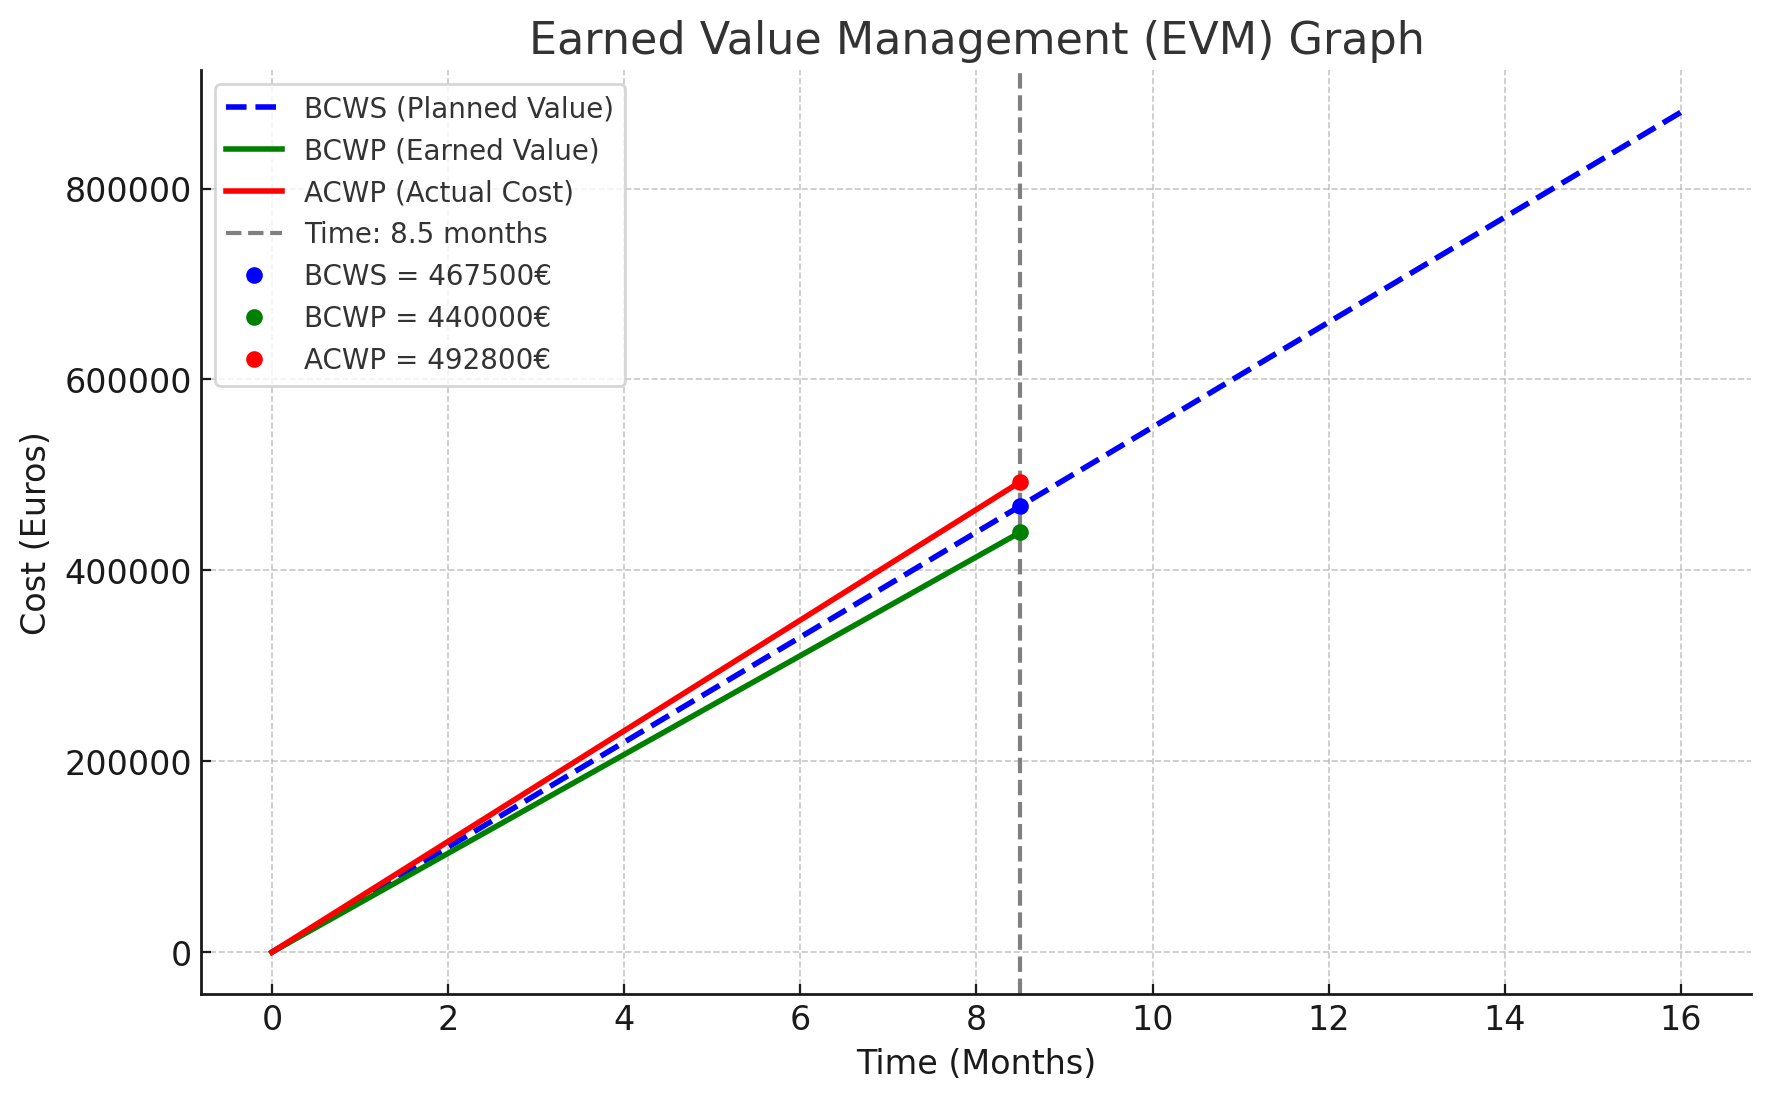
\includegraphics[width=0.9\linewidth]{image.png} % Adjust width to make the image larger
    \caption{Project Schedule} % Add a meaningful caption
    \label{fig:schedule} % Label for referencing the figure
\end{figure}

\subsection*{1. Budget at Completion (BAC)}
The Budget at Completion (BAC) is the total project budget:
\[
\text{BAC} = 220,000 \, \text{euros/phase} \times 4 \, \text{phases} = 880,000 \, \text{euros}
\]

\subsection*{2. BCWS (Budget Cost of Work Scheduled or Planned Value) at 8.5 Months}
The Planned Value (BCWS) is calculated as follows:
\begin{align*}
\text{BCWS} & = (220,000 \, \text{euros} \times 2) + \left( 220,000 \, \text{euros} \times \left( \frac{0.5}{4}=0.125 \right) \right) \\
& = 440,000 \, \text{euros} + 27,500 \, \text{euros} \\
& = 467,500 \, \text{euros}
\end{align*}
The expression \( \frac{0.5}{4} \) is used to calculate the proportion of work planned to be completed by 8.5 months into the project:


\subsection*{3. ACWP (Actual Cost of Work Performed)}
The Actual Cost (ACWP) includes the cost overrun of 12\%. It is calculated as:
\[
\text{ACWP} = 440,000 \, \text{euros} \times (1 + 0.12) = 440,000 \times 1.12 = 492,800 \, \text{euros}
\]

\subsection*{4. BCWP (Earned Value)}

The Earned Value (BCWP) is the value of work completed and is calculated as follows:
\[
\text{BCWP} = \text{BAC} \times \text{Percentage of Work Completed}
\]

Given that:
\begin{itemize}
    \item \(\text{BAC} = 880,000 \, \text{euros}\)
    \item \(\text{Percentage of Work Completed} = 50\% = 0.50\)
\end{itemize}

Thus, the calculation is:
\[
\text{BCWP} = 880,000 \, \text{euros} \times 0.50 = 440,000 \, \text{euros}
\]

Therefore, the BCWP is \( 440,000 \, \text{euros} \), indicating the value of the work completed by the 8.5-month mark.



\subsection*{5. CV (Cost Variance)}
The Cost Variance (CV) is calculated as:
\[
\text{CV} = \text{BCWP} - \text{ACWP}
\]
\[
\text{CV} = 440,000 - 492,800 = -52,800 \, \text{euros}
\]
A negative CV indicates that the project is over budget.

\subsection*{6. SV (Schedule Variance)}
The Schedule Variance (SV) is calculated as:
\[
\text{SV} = \text{BCWP} - \text{BCWS}
\]
\[
\text{SV} = 440,000 - 467,500 = -27,500 \, \text{euros}
\]
A negative SV is unfavorable indicating that the project is behind schedule.

\subsection*{7. CPI (Cost Performance Index)}
The Cost Performance Index (CPI) is calculated as:
\[
\text{CPI} = \frac{\text{BCWP}}{\text{ACWP}}
\]
\[
\text{CPI} = \frac{440,000}{492,800} = 0.8926
\]
A CPI of less than 1 means the project is not cost-efficient.

\section*{8. EAC (Estimate at Completion)}
The Estimate at Completion (EAC) is calculated as:
\[
\text{EAC} = \text{ACWP} + (\text{BAC} - \text{BCWP})
\]
\[
\text{EAC} = 492,800 + (880,000 - 440,000) = 492,800 + 440,000 = 932,800 \, \text{euros}
\]
This means the project is expected to cost 932,800 euros to complete, which is 52,800 euros over the original budget.

\subsection*{Summary of Calculations}

\begin{table}[h!]
    \centering
    \begin{tabular}{|l|l|}
        \hline
        \textbf{Calculation} & \textbf{Value} \\ 
        \hline
        BAC (Budget at Completion) & 880,000 euros \\ 
        \hline
        BCWS (Planned Value) & 467,500 euros \\ 
        \hline
        ACWP (Actual Cost) & 492,800 euros \\ 
        \hline
        BCWP (Earned Value) & 440,000 euros \\ 
        \hline
        CV (Cost Variance) & -52,800 euros \\ 
        \hline
        SV (Schedule Variance) & -27,500 euros \\ 
        \hline
        CPI (Cost Performance Index) & 0.8926 \\ 
        \hline
        EAC (Estimate at Completion) & 932,800 euros \\ 
        \hline
    \end{tabular}
    \caption{Summary of Earned Value Calculations}
\end{table}


\end{document}
